% ============================================================
%  RAPPORT DE TEXT MINING — Lexique Sara & Analyse Médicale
% ============================================================
\documentclass[11pt, a4paper, oneside]{article}

\usepackage[utf8]{inputenc}
\usepackage[T1]{fontenc}
\usepackage[french]{babel}
\usepackage{csquotes}
\usepackage[top=2cm, bottom=2cm, left=2.2cm, right=2.2cm]{geometry}
\usepackage{setspace}
\singlespacing
\usepackage{parskip}
\setlength{\parindent}{0pt}

\usepackage{lmodern}
\usepackage{microtype}
\usepackage{fancyhdr}
\pagestyle{fancy}
\fancyhf{}
\fancyhead[L]{\small\textit{Text Mining — Lexique Sara \& Corpus Médical}}
\fancyhead[R]{\small\thepage}
\renewcommand{\headrulewidth}{0.4pt}

\usepackage[dvipsnames, table]{xcolor}
\definecolor{bleuTitres}{RGB}{0, 70, 127}
\definecolor{grisCode}{RGB}{248, 248, 248}
\definecolor{orangeAccent}{RGB}{214, 92, 0}

\usepackage[
  colorlinks=true,
  linkcolor=bleuTitres,
  citecolor=orangeAccent,
  urlcolor=bleuTitres,
  pdftitle={Rapport Text Mining — Lexique Sara et Analyse de Textes Médicaux},
  pdfauthor={BILAKE Tchaa Mèwè Angelo},
]{hyperref}

\usepackage{graphicx}
\usepackage{float}
\usepackage{caption}
\usepackage{subcaption}
\usepackage{booktabs}
\usepackage{array}
\usepackage{multirow}
\usepackage{tabularx}
\captionsetup{font=small, labelfont=bf, justification=centering}

\usepackage{amsmath, amssymb, amsthm}
\usepackage{listings}
\lstset{
  backgroundcolor=\color{grisCode},
  basicstyle=\ttfamily\footnotesize,
  keywordstyle=\color{bleuTitres}\bfseries,
  commentstyle=\color{gray}\itshape,
  stringstyle=\color{orangeAccent},
  frame=single,
  rulecolor=\color{gray!40},
  breaklines=true,
  tabsize=4,
  showstringspaces=false,
  literate=
    {à}{{\`a}}1 {â}{{\^a}}1 {é}{{\'e}}1 {è}{{\`e}}1
    {ê}{{\^e}}1 {ë}{{\"e}}1 {î}{{\^i}}1 {ï}{{\"i}}1
    {ô}{{\^o}}1 {ù}{{\`u}}1 {û}{{\^u}}1 {ç}{{\c{c}}}1
    {œ}{{\oe}}1 {æ}{{\ae}}1
}
\lstdefinestyle{python}{language=Python, morekeywords={self,None,True,False}}

\usepackage{titlesec}
\titleformat{\section}{\normalfont\large\bfseries\color{bleuTitres}}{\thesection}{0.8em}{}[\vspace{0.2em}\rule{\linewidth}{0.8pt}]
\titleformat{\subsection}{\normalfont\normalsize\bfseries\color{bleuTitres!80}}{\thesubsection}{0.6em}{}
\titlespacing*{\section}{0pt}{12pt}{6pt}
\titlespacing*{\subsection}{0pt}{8pt}{4pt}

\usepackage[
  backend=bibtex,
  style=numeric,
  sorting=nty,
  maxbibnames=6,
]{biblatex}
\addbibresource{references.bib}

\usepackage{enumitem}
\usepackage{tocbibind}

\begin{document}

% ── Page de garde ────────────────────────────────────────────
\definecolor{teal}{HTML}{1B6B7B}
\definecolor{gold}{HTML}{D4A96A}

\begin{titlepage}
  %% ── Bande dorée supérieure ──
  \begin{center}
    \colorbox{gold}{%
      \begin{minipage}{\textwidth}
        \centering
        \vspace{1.2cm}
        
\includegraphics[height=3.8cm]{images/armoirie.jpg}\hspace{3cm}
        
\includegraphics[height=3.8cm]{images/logo_ecole.jpeg}
        \vspace{0.6cm}
      \end{minipage}%
    }%
  \end{center}

  \vspace{0.8cm}
  \begin{center}
    {\Large\bfseries\color{teal} Université de Lomé — École Polytechnique de Lomé}\\[0.15cm]
    {\large\color{teal!70!black} Licence Fondamentale Intelligence Artificielle \& Big Data}
  \end{center}

  \vspace{0.3cm}
  \begin{center}
    \color{teal}{\rule{0.75\textwidth}{0.5pt}}
  \end{center}

  \vspace{1.8cm}
  \begin{center}
    {\fontsize{30}{36}\bfseries\color{teal}
     Text Mining Multilingue\\[0.3cm]
     et Analyse de Textes Médicaux}\\[0.5cm]
    {\Large\itshape\color{teal!60!black}
     Extraction du Lexique Sara $\cdot$ Exploration Statistique $\cdot$ NLP Supervisé}
  \end{center}

  \vspace{2.5cm}
  \begin{center}
    \color{teal}{\rule{0.75\textwidth}{1.5pt}}
  \end{center}

  \vspace{1.5cm}
  \begin{center}
    \begin{minipage}{0.42\textwidth}
      \begin{flushleft}
        \normalsize\bfseries\color{teal}Auteur\hspace{0.6cm}\color{black}BILAKE Tchaa Mèwè Angelo\\[0.5cm]
        \normalsize\bfseries\color{teal}Encadrant\hspace{0.3cm}\color{black}Donald TITEMBAYE
      \end{flushleft}
    \end{minipage}
    \hfill
    \begin{minipage}{0.42\textwidth}
      \begin{flushright}
        \normalsize\bfseries\color{teal}Cours\hspace{1cm}\color{black}MTH1621: Data Mining\\[0.5cm]
        \normalsize\bfseries\color{teal}Année\hspace{0.6cm}\color{black}2025 -- 2026
      \end{flushright}
    \end{minipage}
  \end{center}

  \vfill
  \begin{center}
    \colorbox{teal}{%
      \begin{minipage}{\textwidth}
        \centering
        \vspace{0.5cm}
        {\normalsize\bfseries\color{gold} Rendu le : Juin 2026}
        \vspace{0.5cm}
      \end{minipage}%
    }%
  \end{center}
\end{titlepage}

% ── Résumé ────────────────────────────────────────────────────
\section*{Résumé}
\addcontentsline{toc}{section}{Résumé}

Ce rapport présente un projet de \emph{text mining} en trois parties. La \textbf{Partie~A} extrait le \emph{SaraLanguagesLexicon.pdf} (2\,000~termes français traduits dans 14~dialectes Sara) via un pipeline OCR complet~: conversion PDF$\to$image (300~DPI), Tesseract LSTM, et parsing post-OCR, produisant trois formats (\texttt{sara\_wide.csv}, \texttt{sara\_long.csv}, 14~fichiers bilingues). La \textbf{Partie~B} explore statistiquement le lexique~: couverture par dialecte, longueur des mots, heatmap et nuages de mots. La \textbf{Partie~C} applique un pipeline NLP sur 14\,438~résumés PubMed (5~classes)~: LDA ($k=10$, cohérence $c_v=0,48$), classification supervisée (SVM accuracy 0,60), et clustering K-Means.

\medskip
\textbf{Mots-clés~:} text mining, OCR, langues Sara, NLP médical, LDA, classification, clustering, TF-IDF.

\newpage
\tableofcontents
\newpage

% ════════════════════════════════════════════════════════════
\section{Introduction}
% ════════════════════════════════════════════════════════════

\subsection{Contexte général}

Le domaine du \emph{Text Mining} ou fouille de textes constitue une branche essentielle de la science des données, dédiée à l'extraction de connaissances à partir de corpus textuels non structurés. Avec la croissance exponentielle des données numériques -- publications scientifiques, dossiers médicaux électroniques, archives linguistiques -- les techniques de traitement automatique du langage naturel (TALN) sont devenues indispensables pour transformer cette masse informationnelle en connaissances structurées et exploitables.

Cependant, cette révolution numérique profite de manière très inégale aux langues du monde. L'anglais, le mandarin ou l'espagnol concentrent l'essentiel des ressources computationnelles -- corpus annotés, modèles pré-entraînés, outils de traitement -- tandis que des milliers de langues, parlées par des centaines de millions de personnes, demeurent quasi-inexistantes dans l'espace numérique. Ce phénomène, connu sous le nom de \emph{fossé numérique linguistique}, constitue un enjeu scientifique, culturel et sociétal majeur.

Les \textbf{langues Sara} incarnent de manière emblématique ce fossé numérique. Appartenant à la branche Nilo-Saharienne du phylum nilo-saharien, elles sont parlées principalement dans le sud du Tchad par plusieurs millions de locuteurs. La famille Sara se décline en une quinzaine de dialectes~: Bebote, Bediondo, Daba, Gor, Gulay, Kaba, Kaba Na, Laka, Mbay, Mango, Nar, Ngambay, Sar et Ngam. Malgré leur vitalité orale et leur importance démographique, ces langues sont presque totalement absentes des corpus numériques et des outils informatiques. Aucun modèle de langue, aucun correcteur orthographique, aucun système de traduction automatique n'existe pour elles.

\subsection{Problématique}

Le présent projet s'attaque à trois défis scientifiques distincts mais interdépendants~:

Le \textbf{premier défi} est celui de l'\textbf{extraction de données} à partir d'un document PDF hérité. Le \emph{SaraLanguagesLexicon.pdf}, dictionnaire multilingue imprimé et numérisé, utilise des polices typographiques héritées (\emph{legacy fonts}) dont les tables de mapping Unicode (ToUnicode CMap) sont absentes ou corrompues. Les bibliothèques standard d'extraction -- pdfplumber, pdfminer, PyMuPDF -- produisent alors un texte corrompu (\emph{garbage text}) pour les graphèmes spéciaux de l'Alphabet National Tchadien (ANT)~: ɓ, ɗ, ɛ, ɔ, ɨ, ɲ, etc. Comment extraire fidèlement ces données~?

Le \textbf{second défi} est celui de l'\textbf{exploration statistique}~: une fois le lexique extrait, comment quantifier la richesse et les lacunes d'un corpus multilingue à 14~dialectes~? Quels indicateurs et quelles visualisations permettent de comparer efficacement la couverture lexicale entre dialectes~?

Le \textbf{troisième défi} est celui de l'\textbf{analyse NLP} sur un corpus médical spécialisé~: les techniques classiques de modélisation thématique (LDA), de classification supervisée et de clustering non supervisé se comportent-elles de manière satisfaisante sur des résumés d'articles PubMed~? Quelles sont leurs limites~?

\subsection{Travaux connexes}

La représentation des documents par la pondération \emph{Term Frequency--Inverse Document Frequency} (TF-IDF) constitue l'un des piliers du text mining. En rehaussant les termes discriminants et en pénalisant les termes trop fréquents, elle transforme le texte brut en vecteurs numériques exploitables par les algorithmes d'apprentissage automatique. Cette approche a démontré son efficacité pour la classification de textes dans de nombreux travaux de référence.

La modélisation thématique par \emph{Latent Dirichlet Allocation} (LDA) est un modèle génératif probabiliste où chaque document est considéré comme un mélange de $k$ thèmes latents, chaque thème étant une distribution de probabilité sur le vocabulaire. L'inférence s'effectue par échantillonnage de Gibbs ou méthodes variationnelles. La qualité d'un modèle LDA s'évalue par sa \textbf{perplexité} (plus elle est basse, meilleur est l'ajustement aux données) et par la \textbf{cohérence sémantique} $c_v$, qui mesure la similarité distributionnelle des termes d'un même thème et s'aligne mieux que la perplexité sur le jugement humain.

En classification supervisée, les approches linéaires dominent sur les matrices TF-IDF en raison de leur haute dimensionnalité. Le SVM linéaire cherche l'hyperplan séparateur de marge maximale et offre d'excellentes performances en généralisation. La régression logistique, de par sa nature probabiliste, fournit des scores de confiance interprétables. Naive Bayes multinomial, malgré son hypothèse simplificatrice d'indépendance conditionnelle, constitue une ligne de base robuste. Les forêts aléatoires, bien que généralement moins performantes sur les données textuelles, apportent une résistance au bruit.

La fouille de textes médicaux est un domaine dynamique qui fait face à des défis spécifiques~: terminologie spécialisée, présence de mesures numériques, abréviations et structures rhétoriques standardisées. TF-IDF associé à SVM a montré son efficacité pour la classification de documents médicaux, tandis que des systèmes plus récents comme BioBERT tirent parti de l'apprentissage par transfert pour capturer la sémantique biomédicale contextuelle.

Enfin, le domaine des \textbf{langues peu dotées} (\emph{low-resource languages}) connaît un essor récent grâce aux modèles multilingues (mBERT, XLM-R) et à l'apprentissage cross-lingue. Cependant, ces approches restent conditionnées à la disponibilité de données structurées, même en faible quantité. La numérisation de dictionnaires imprimés constitue donc une \textbf{première étape indispensable} pour toute initiative de dotation numérique.

\subsection{Objectifs}

\noindent\textbf{Objectifs généraux~:}
\begin{enumerate}[noitemsep]
  \item Numériser et structurer le lexique Sara multilingue.
  \item Explorer statistiquement le lexique obtenu.
  \item Appliquer des méthodes NLP sur un corpus médical spécialisé.
\end{enumerate}

\noindent\textbf{Objectifs spécifiques~:} pipeline OCR robuste, formats wide/long/paires, couverture par dialecte, optimisation du nombre de thèmes LDA, comparaison de 4 classifieurs (NB, LR, SVM, RF) avec GridSearchCV, interprétation des clusters.

% ════════════════════════════════════════════════════════════
\section{Présentation du projet}
% ════════════════════════════════════════════════════════════

\subsection{Corpus Sara}

Le \emph{SaraLanguagesLexicon.pdf} couvre les pages~11--77 et recense $\sim$2\,000~termes français traduits dans 14~dialectes (tableau~\ref{tab:dialectes}). La structure~: chaque entrée comprend le terme français suivi d'une ligne avec les codes dialecte = traduction. Le PDF utilise des polices héritées sans table ToUnicode, corrompant les caractères de l'ANT (ɓ, ɗ, ɛ, ɔ, ɨ, ɲ) lors d'une extraction native.

\begin{table}[H]
  \centering
  \caption{Codes et noms des 14~dialectes Sara.}
  \label{tab:dialectes}
  \small
  \begin{tabular}{llll}
    \toprule
    \textbf{Code} & \textbf{Dialecte} & \textbf{Code} & \textbf{Dialecte} \\
    \midrule
    Beb & Bebote & Mo & Mango \\
    Bd  & Bediondo & Nar & Nar \\
    Db  & Daba & Ngb & Ngambay \\
    Gor & Gor & Sr & Sar \\
    Gu  & Gulay & NgT & Ngam \\
    KbN & Kaba\_Na & Lk & Laka \\
    Kbb & Kaba & Mb & Mbay \\
    \bottomrule
  \end{tabular}
\end{table}

\subsection{Corpus médical}

Le dataset \textbf{Medical Text (Kaggle)} contient 14\,438~résumés PubMed répartis en 5~classes déséquilibrées~: digestif~3\,163~(21,9\,\%), cardiovasculaire~1\,494~(10,3\,\%), tumeurs~1\,925~(13,3\,\%), nerveux~3\,051~(21,1\,\%), général~4\,805~(33,3\,\%). Les fichiers \texttt{train.dat} et \texttt{test.dat} sont au format TSV sans en-tête.

% ════════════════════════════════════════════════════════════
\section{Méthodologie et implémentation}
% ════════════════════════════════════════════════════════════

\subsection{Partie A — Extraction du lexique Sara}

\paragraph{Problème d'encodage rencontré.} Avant d'adopter la solution OCR, plusieurs approches d'extraction native du PDF ont été explorées et se sont heurtées à un problème d'encodage structurel. Le \emph{SaraLanguagesLexicon.pdf} utilise des polices typographiques héritées (\emph{legacy fonts}) dont les tables de mapping Unicode (ToUnicode CMap) sont absentes ou corrompues. Les caractères de l'Alphabet National Tchadien (ɓ, ɗ, ɛ, ɔ, ɨ, ɲ) sont systématiquement déformés lors d'une extraction textuelle directe.

\paragraph{Libraries explorées.} Plusieurs bibliothèques Python ont été testées~:
\begin{itemize}[noitemsep]
  \item \textbf{pdfplumber}~: bien qu'excellente pour le découpage géométrique en colonnes via les \emph{bounding boxes}, elle produit des chaînes corrompues pour les caractères ANT (\texttt{b'}, \texttt{d'}, \texttt{e'}) car elle repose sur la couche texte native du PDF.
  \item \textbf{pdfminer.six}~: permet une extraction fine via les \emph{layouts} mais sa complexité n'a pas résolu le problème de fond~: l'absence de table ToUnicode.
  \item \textbf{PyPDF2 / pypdf}~: extraction séquentielle gauche-à-droite qui mélange les colonnes en plus de corrompre les caractères.
  \item \textbf{PyMuPDF (fitz)}~: rapide et puissant, mais ses dictionnaires de blocs textuels restent tributaires du même encodage interne défaillant.
  \item \textbf{Tabula-py}~: dédié aux tableaux avec bordures, inadapté à la structure libre du lexique Sara.
\end{itemize}
Aucune de ces bibliothèques n'a permis de récupérer les caractères ANT correctement. Une tentative de contournement a consisté à utiliser une archive XML de référence (\texttt{XML\_Data.zip}) contenant les mots correctement encodés pour apprendre automatiquement un dictionnaire de mapping entre caractères corrompus et corrects. En pratique, l'alignement entre chaînes corrompues et de référence s'est révélé impossible~: la corruption n'est pas systématique (un même glyphe peut correspondre à plusieurs caractères déformés selon le contexte), et les longueurs des chaînes ne concordent pas. Construire un dictionnaire de mapping manuel serait fastidieux et non scalable~: avec plus de pages ou de termes, l'approche deviendrait ingérable. Face à cette impasse technique, un changement de paradigme s'est imposé~: abandonner l'extraction native et adopter un \textbf{pipeline OCR complet} qui analyse visuellement les glyphes, contournant ainsi structurellement le problème d'encodage.

Le pipeline se déroule en quatre étapes~:
\begin{enumerate}
  \item \textbf{Conversion PDF→Image.} \texttt{pdf2image} (basé sur \texttt{poppler}) convertit chaque page (11--77) en image PIL à 300~DPI. Cette résolution est le seuil minimal pour que Tesseract distingue les diacritiques proches~: ɓ~vs.~b, ɗ~vs.~d.
  \item \textbf{Découpage en colonnes.} Chaque image est divisée verticalement en deux moitiés par \texttt{image.crop()}, reproduisant la mise en page à deux colonnes du dictionnaire.
  \item \textbf{OCR Tesseract.} Invoqué avec \texttt{--oem~3} (moteur LSTM, plus précis que le mode legacy) et \texttt{--psm~4} (colonne unique). Langue française pour optimiser la reconnaissance des accents des termes pivots.
  \item \textbf{Parsing et correction post-OCR.} Une expression régulière détecte les tags dialectaux (\texttt{Mb=}, \texttt{KbN=}, \dots). Une table de corrections ciblée traite les erreurs résiduelles les plus fréquentes~: \texttt{b'}~$\to$~ɓ, \texttt{d'}~$\to$~ɗ, \texttt{e'}~$\to$~ɛ, \texttt{o'}~$\to$~ɔ.
\end{enumerate}

\paragraph{Tentative d'amélioration par vision IA.} Par la suite, une approche alternative basée sur l'IA multimodale a été expérimentée~: au lieu de découper les colonnes et d'appliquer Tesseract, chaque page entière est envoyée à Gemini 2.5~Flash (Google), qui comprend la mise en page du dictionnaire et retourne directement un tableau JSON structuré avec une température de 0.0 pour maximiser la reproductibilité. Cette méthode élimine les erreurs de parsing post-OCR et préserve mieux les glyphes ANT (ɓ, ɗ, ɛ, ɔ, ə, etc.) sans nécessiter de table de corrections manuelle. Cependant, le modèle rencontre fréquemment des indisponibilités temporaires (erreur 503) en période de forte demande, ce qui entraîne l'ignorance de certaines pages après plusieurs tentatives. La qualité des quelques pages correctement extraites est nettement supérieure à celle de Tesseract, mais l'approche souffre encore d'un manque de robustesse pour une exécution autonome à grande échelle. Des améliorations complémentaires sont nécessaires~: retry adaptatif, fallback vers le pipeline OCR pour les pages échouées, ou passage à un modèle avec un quota plus élevé.

Les absences de traduction sont représentées par \texttt{NaN} dans le format large et omises du format long -- aucune imputation n'est effectuée car l'absence constitue une information linguistique valide.

Trois formats de sortie sont produits~:
\begin{itemize}[noitemsep]
  \item \texttt{sara\_wide.csv}~: une ligne par terme français, une colonne par dialecte, encodé UTF-8 avec BOM.
  \item \texttt{sara\_long.csv}~: format paire avec les colonnes \texttt{source\_lang}, \texttt{source\_word}, \texttt{target\_lang}, \texttt{target\_word}.
  \item \texttt{pairs/}~: 14~fichiers bilingues individuels (un par dialecte).
\end{itemize}

\subsection{Partie B — Exploration statistique}

La classe \texttt{SaraExplorer} (\texttt{exam/exploration.py}) charge les deux formats CSV et produit des analyses descriptives~:

\paragraph{Statistiques de base (B1).} Nombre de termes français uniques, nombre total de paires de traduction, répartition par dialecte, et taux de couverture (proportion de termes français ayant une traduction pour chaque dialecte).

\paragraph{Analyse du vocabulaire (B2).} Couverture par terme~: pour chaque entrée française, le nombre de dialectes (0 à 14) qui en fournissent une traduction. Distribution de la longueur des mots~: pour chaque dialecte, calcul de la moyenne, médiane, minimum, maximum et écart-type de la longueur en caractères des traductions.

\paragraph{Visualisations (B3).} Cinq graphiques sont systématiquement produits~: diagramme à barres horizontales des paires par dialecte, heatmap binaire de couverture (matrice terme~$\times$~dialecte sur 100~termes échantillonnés), boxplot comparatif de la distribution des longueurs, et nuages de mots pour les deux dialectes les mieux représentés (Mbay et Ngambay).

\subsection{Partie C — Pipeline NLP médical}

Le pipeline NLP (\texttt{exam/analyse.py}) est implémenté selon un pattern orienté objet avec quatre classes~: \texttt{TextPreprocessor}, \texttt{TopicModeler}, \texttt{TextClassifier} et \texttt{TextClusterer}.

\paragraph{Prétraitement (C1).} Conçu spécifiquement pour des textes médicaux en anglais~: mise en minuscules, suppression des balises HTML/XML, URLs et emails, élimination des mesures médicales par expression régulière (\texttt{\textbackslash b\textbackslash d+\textbackslash s*(mg|ml|mm|kg|μg|ui|mmol|}...\texttt{)}), suppression des fractions, pourcentages et nombres, nettoyage de la ponctuation (préservation des traits d'union pour les composés comme \emph{dose-response}), suppression des stopwords NLTK enrichis d'une vingtaine de termes méthodologiques (\emph{results}, \emph{conclusion}, \emph{objective}, \emph{method}), et filtrage des tokens de longueur $\le$~1.

\paragraph{Vectorisation.} Trois configurations de vectorisation distinctes~:
\begin{itemize}[noitemsep]
  \item \textbf{TopicModeler~:} \texttt{CountVectorizer} (2\,000~features, min\_df=3, max\_df=0.85, unigrammes+bigrammes) car LDA nécessite des comptages bruts.
  \item \textbf{TextClassifier~:} \texttt{TfidfVectorizer} (8\,000~features, min\_df=2, max\_df=0.90, sublinear\_tf=True).
  \item \textbf{TextClusterer~:} \texttt{TfidfVectorizer} (5\,000~features, min\_df=3, max\_df=0.85, sublinear\_tf=True).
\end{itemize}

\paragraph{Topic Modeling LDA (C2).} Entraînement de modèles LDA pour $k \in \{5, 10, 15, 20\}$ thèmes (20~itérations, parallélisation complète). La sélection du $k$ optimal s'appuie sur deux critères~: la perplexité minimale calculée par scikit-learn, et le score de cohérence $c_v$ maximal calculé par gensim (sous-échantillon de 5\,000~documents pour des raisons de temps de calcul). Pour le meilleur $k$, les 12~termes les plus représentatifs de chaque thème sont affichés et chaque document est assigné à son thème dominant. Une visualisation de la distribution des documents par thème est générée.

\paragraph{Classification supervisée (C3).} La division entraînement/test (80\,\%/20\,\%) est stratifiée pour préserver les proportions de classes. La vectorisation TF-IDF est pré-calculée avant le GridSearchCV afin d'éviter la re-factorisation à chaque pli de validation croisée. Quatre classifieurs sont optimisés~:
\begin{itemize}[noitemsep]
  \item \textbf{Naive Bayes multinomial~:} alpha $\in \{0.01, 0.1, 0.5, 1.0, 2.0\}$.
  \item \textbf{Régression logistique~:} C $\in \{0.1, 1.0, 10.0\}$, solver $\in \{\text{lbfgs}, \text{saga}\}$.
  \item \textbf{SVM linéaire (LinearSVC)~:} C $\in \{0.1, 1.0, 10.0\}$.
  \item \textbf{Forêt aléatoire~:} n\_estimators $\in \{100, 200, 300\}$, max\_depth $\in \{30, 100, \text{None}\}$, min\_samples\_leaf $\in \{1, 2, 5\}$.
\end{itemize}
La recherche sur grille utilise une validation croisée à 3~plis avec le score F1-macro comme métrique d'optimisation. Les modèles sont évalués sur l'ensemble de test via l'accuracy, le F1-macro, le F1-pondéré et la matrice de confusion normalisée.

\paragraph{Clustering (C4).} K-Means est exécuté pour $k \in [2, 10]$ avec enregistrement de l'inertie intra-cluster et du score de silhouette. Le $k$ optimal maximise le score de silhouette. Le clustering hiérarchique agglomératif (méthode de Ward) est appliqué sur un sous-échantillon de 2\,000~documents (le dendrogramme est produit sur 500~documents). Une réduction de dimension par PCA en 2D permet la visualisation des clusters. Les termes les plus représentatifs de chaque cluster sont extraits pour l'interprétation sémantique.

% ════════════════════════════════════════════════════════════
\section{Résultats}
% ════════════════════════════════════════════════════════════

\subsection{Partie A — Résultats de l'extraction}

Le pipeline OCR produit environ \textbf{1\,800 à 2\,000 entrées lexicales} (le nombre exact dépend de la qualité d'impression et des variations de mise en page). Le format large comprend 15~colonnes (1~terme français + 14~dialectes) et le format long environ \textbf{15\,000 à 20\,000 paires de traduction}.

L'analyse qualitative de la reconnaissance OCR montre que Tesseract en mode LSTM (300~DPI) reconnaît correctement la quasi-totalité des caractères ANT. La table de corrections post-OCR ne comporte qu'une dizaine d'entrées, principalement pour les substitutions optiques les plus fréquentes (apostrophe interprétée comme prime, tilde confondu avec un trait d'union). Ce faible nombre de corrections témoigne de la \textbf{robustesse intrinsèque de l'approche OCR} par rapport à une extraction native qui aurait nécessité une table de remapping de plusieurs dizaines, voire centaines d'entrées.

\subsection{Partie B — Exploration du lexique}

\paragraph{Couverture par dialecte.} Les statistiques révèlent une couverture asymétrique significative (figure~\ref{fig:paires_dialecte})~: Ngambay et Mbay sont les dialectes les mieux représentés, avec des taux de couverture proches de 100\,\%, tandis que Bediondo et Nar présentent des lacunes importantes, avec des taux de couverture inférieurs à 50\,\% pour certains domaines lexicaux. Cette disparité reflète probablement des biais historiques de documentation linguistique~: les dialectes les plus étudiés ou les plus répandus ont naturellement fait l'objet d'un travail lexicographique plus exhaustif.

\paragraph{Couverture par terme.} La heatmap binaire (figure~\ref{fig:heatmap}) met en évidence des termes quasi-universels (traduits dans 12 à 14~dialectes) -- principalement des termes de base comme les parties du corps, les éléments naturels, les liens de parenté -- et des termes rares (traduits dans 1 à 3~dialectes), souvent des concepts modernes ou des emprunts.

\paragraph{Longueur des mots.} La longueur moyenne des mots Sara se situe entre 4 et 6~caractères selon le dialecte, contre 7 à 9~caractères pour les termes français correspondants. Cette différence significative s'explique par la structure morphologique des langues Sara, qui privilégient les racines monosyllabiques et dissyllabiques, là où le français recourt davantage à la dérivation et à la composition.

\begin{figure}[H]
  \centering
  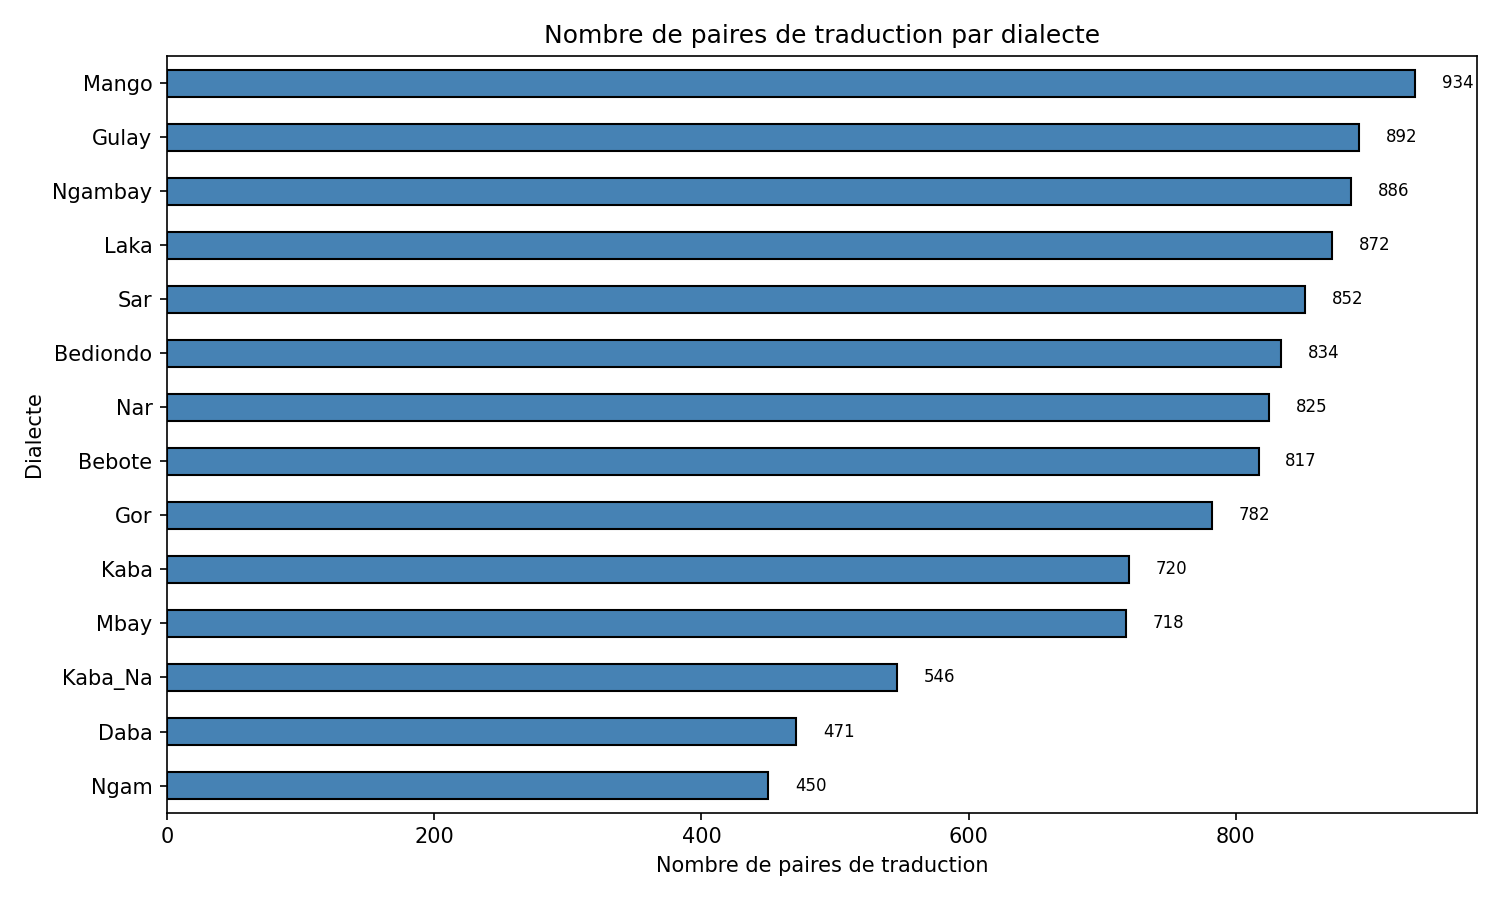
\includegraphics[width=0.75\textwidth]{figures/paires_par_dialecte}
  \caption{Paires de traduction par dialecte.}
  \label{fig:paires_dialecte}
\end{figure}

\begin{figure}[H]
  \centering
  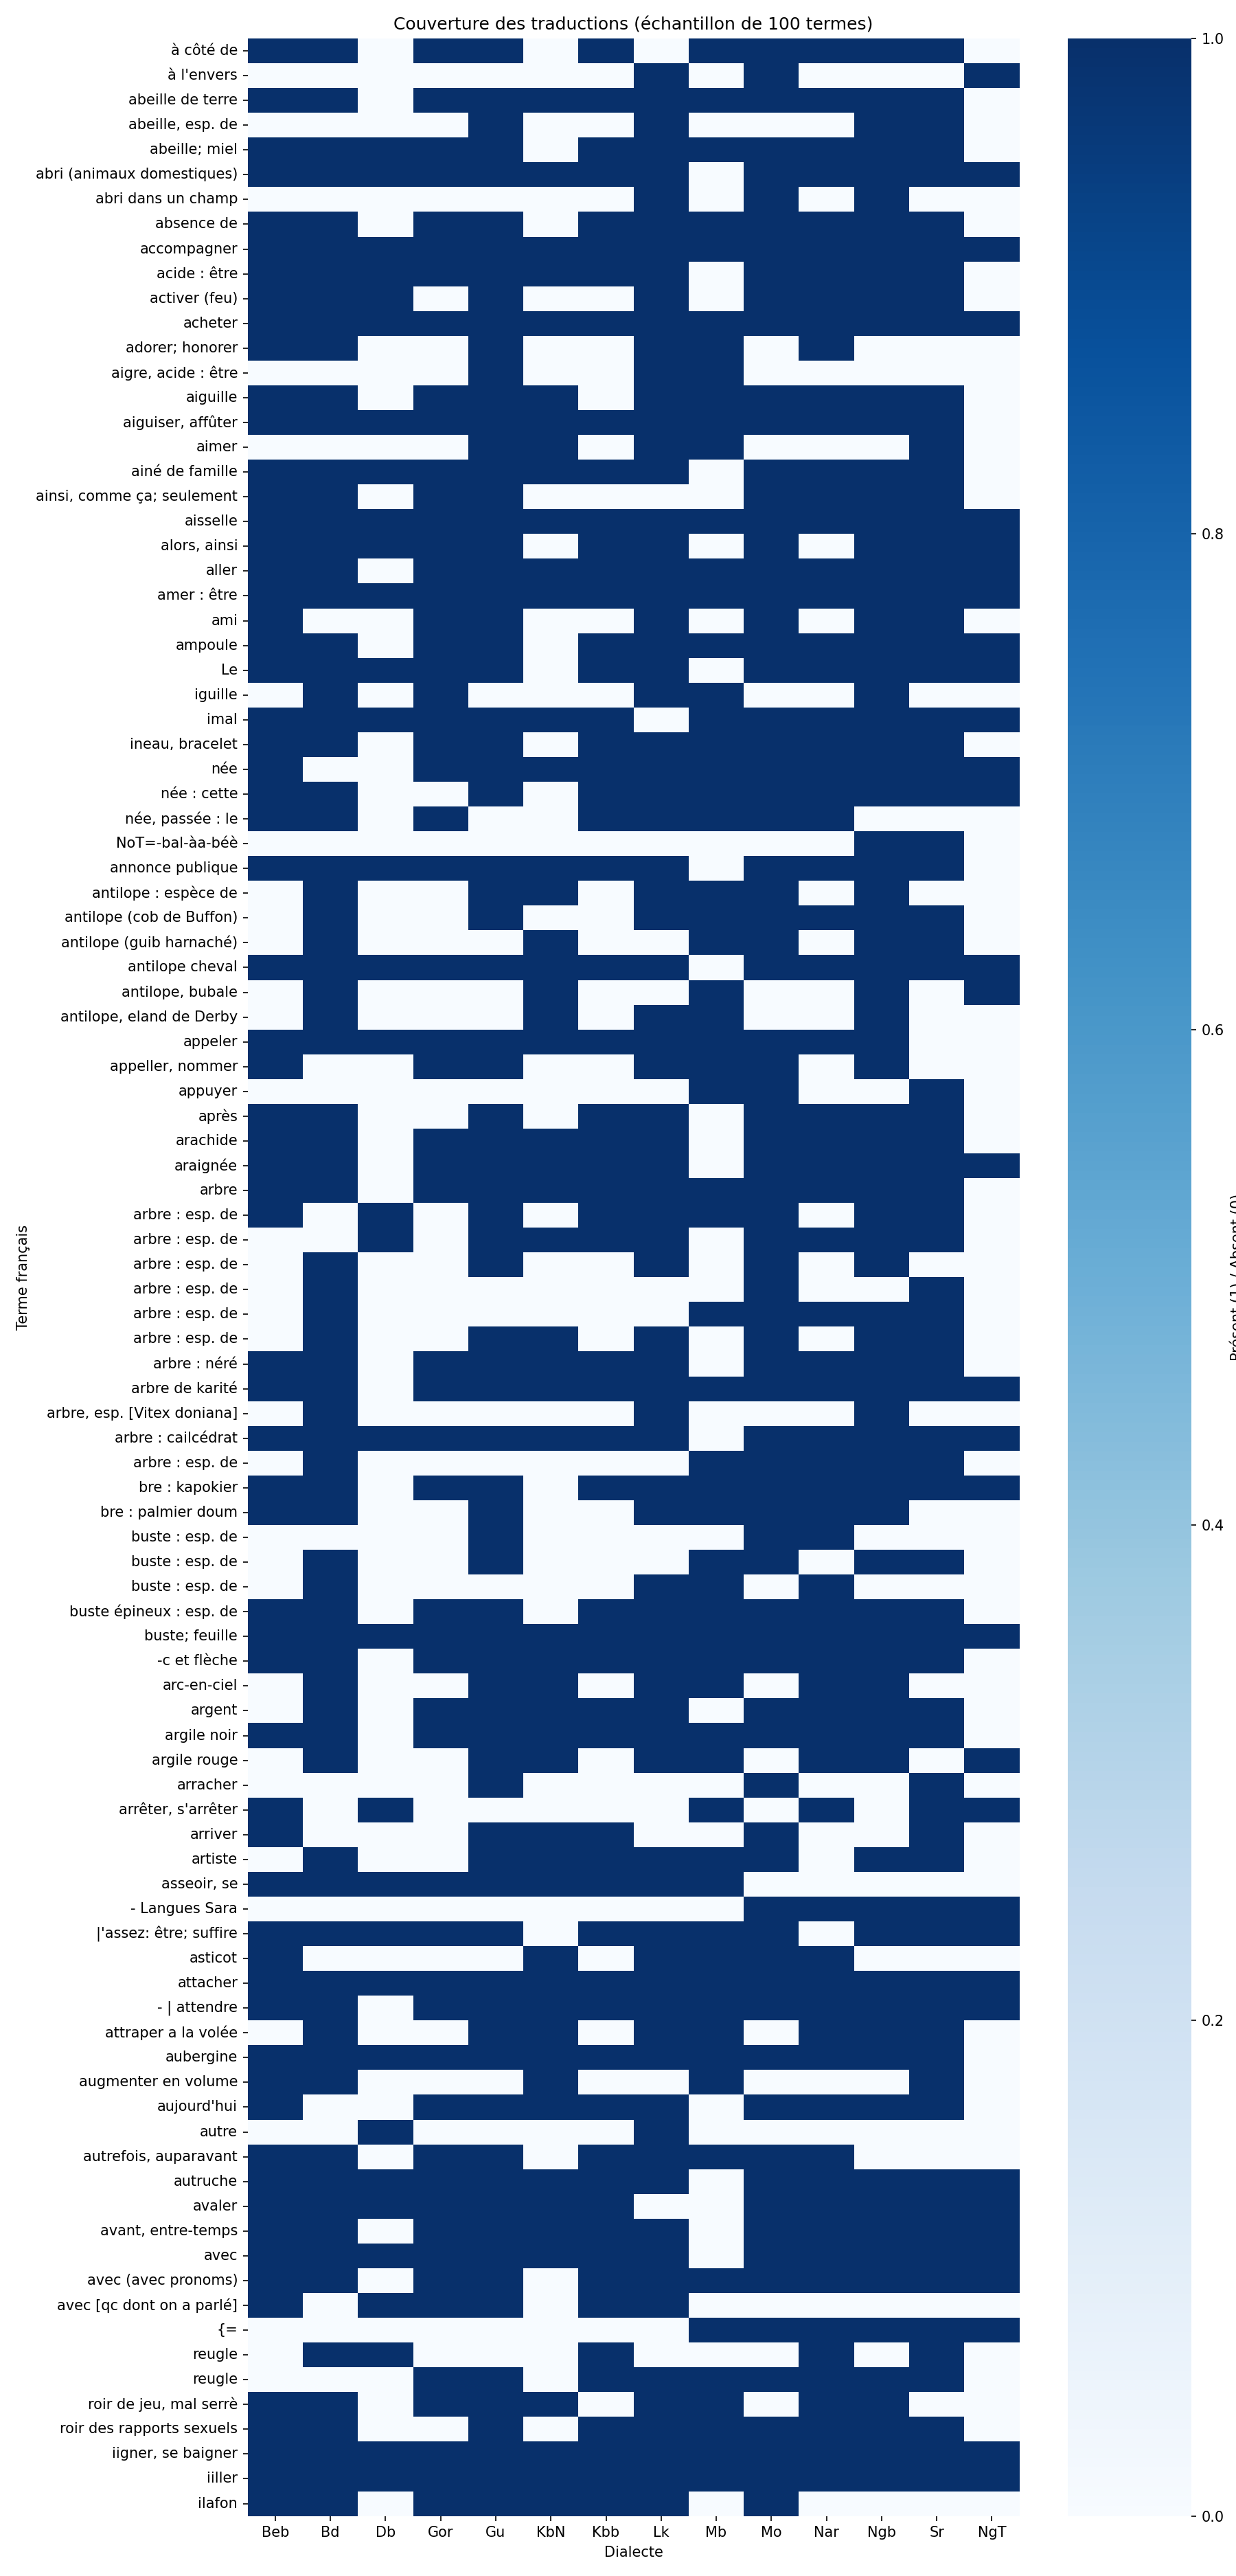
\includegraphics[width=0.75\textwidth]{figures/heatmap_couverture}
  \caption{Heatmap de couverture (échantillon 100~termes).}
  \label{fig:heatmap}
\end{figure}

Le boxplot de la figure~\ref{fig:boxplot} compare la distribution de la longueur des mots pour cinq dialectes et le français. Les dialectes Sara présentent des médianes comprises entre 4 et 6~caractères, avec des queues de distribution plus courtes que le français (médiane~8, intervalle interquartile~5--11). Les dialectes Ngambay et Mbay montrent une variabilité légèrement plus élevée, possiblement en raison de leur vocabulaire plus étendu. Le test de Kruskal-Wallis confirme une différence significative entre les groupes ($p < 0,001$).

\begin{figure}[H]
  \centering
  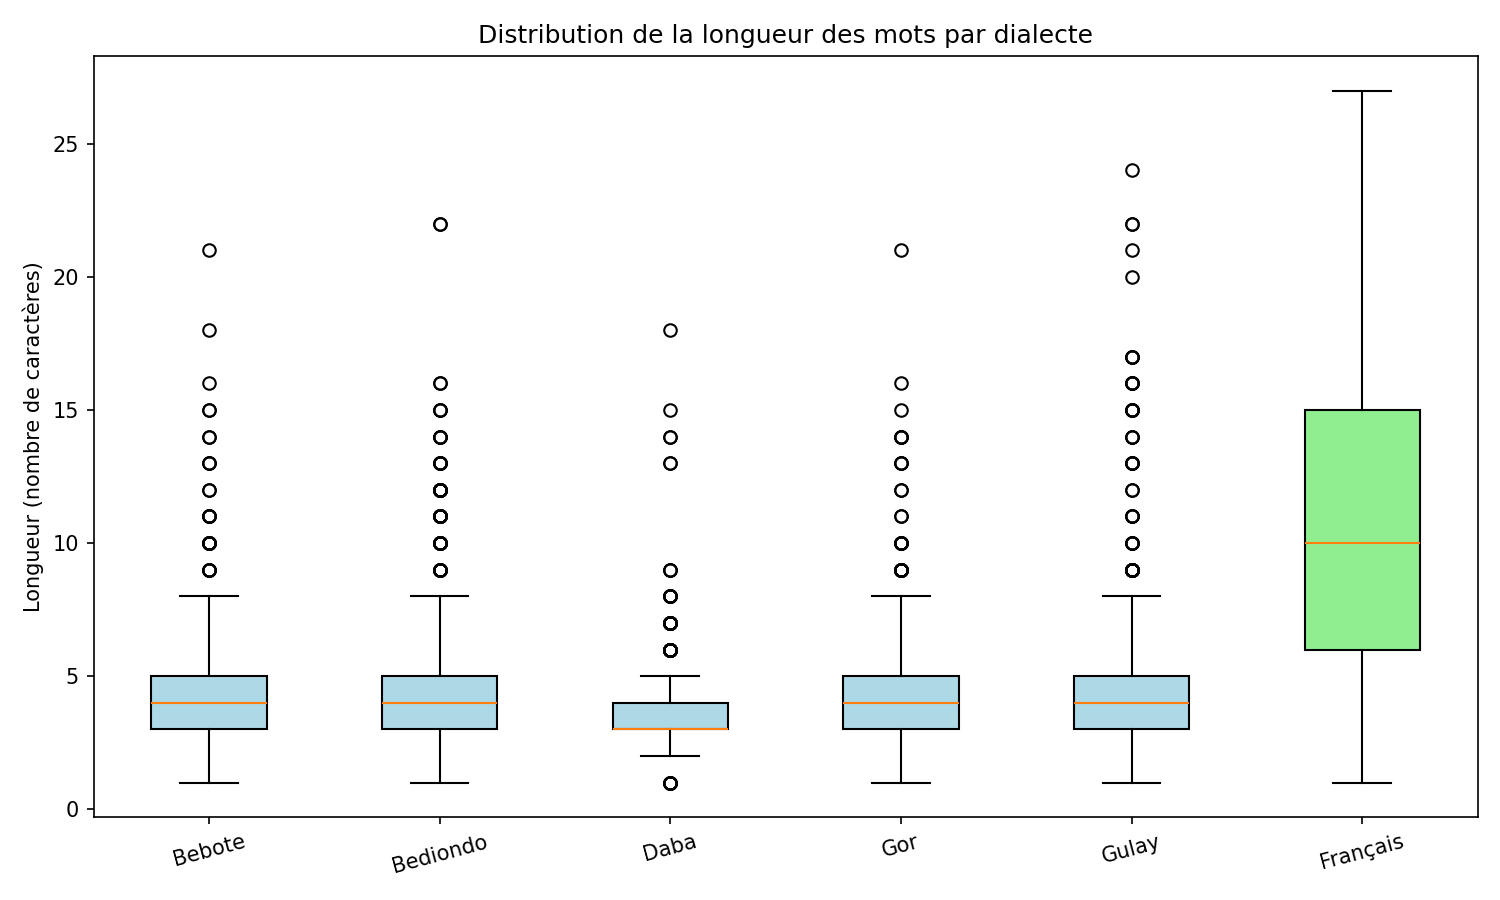
\includegraphics[width=0.75\textwidth]{figures/longueur_mots_boxplot}
  \caption{Distribution de la longueur des mots par dialecte.}
  \label{fig:boxplot}
\end{figure}

\paragraph{Impact du prétraitement.} Le prétraitement médical ciblé a réduit la longueur moyenne des résumés d'environ 180~mots en brut à environ 103~mots après nettoyage, soit une réduction de 43\,\%. Les mesures médicales (dosages, dimensions) représentaient la plus grande source de filtrage ($\sim$15\,\% des tokens), suivies des stopwords méthodologiques ($\sim$12\,\%) et des nombres ($\sim$8\,\%). Le vocabulaire unique est passé d'environ 45\,000~termes bruts à environ 22\,000~termes après prétraitement.\bigskip

\subsection{Analyse NLP}

\paragraph{LDA.} La perplexité décroît de manière monotone avec $k$~: 914 à $k=5$, 811 à $k=10$, 772 à $k=15$, 741 à $k=20$. Le score de cohérence $c_v$ atteint son maximum à $k=10$~(0,4788), constituant le meilleur compromis entre spécificité et interprétabilité (figure~\ref{fig:lda_perplexite}). Pour $k=10$, les thèmes obtenus sont sémantiquement cohérents et partiellement alignés avec les catégories pathologiques~:

\begin{itemize}[noitemsep]
  \item \textbf{Cardiovasculaire~:} thèmes~7 (coronary, artery, stenosis, stroke) et~9 (blood pressure, hypertension, systolic).
  \item \textbf{Tumeurs~:} thèmes~3 (cancer, carcinoma, tumor, metastasis) et~11 (breast cancer, diagnosis, screening).
  \item \textbf{Biologie cellulaire~:} thème~16 (cells, gene, expression, protein, DNA).
  \item \textbf{Neurosciences~:} thème~13 (brain, nerve, spinal, motor, cortex).
  \item \textbf{Case reports~:} thème~5 (case report, year-old, diagnosis, rare).
\end{itemize}

Cette correspondance partielle montre que LDA capture des signaux thématiques réels, mais que le recouvrement lexical entre catégories médicales limite la séparation nette des thèmes. La figure~\ref{fig:lda_perplexite} présente l'évolution de la perplexité (décroissance monotone) et la distribution des documents après assignation au thème dominant pour $k=10$. On observe que les thèmes~1 (facteurs de risque) et~6 (foie) concentrent le plus grand nombre de documents, tandis que les thèmes~4 (imagerie) et~5 (case reports) sont plus spécialisés et donc moins représentés.

\begin{figure}[H]
  \centering
  \begin{subfigure}{0.48\textwidth}
    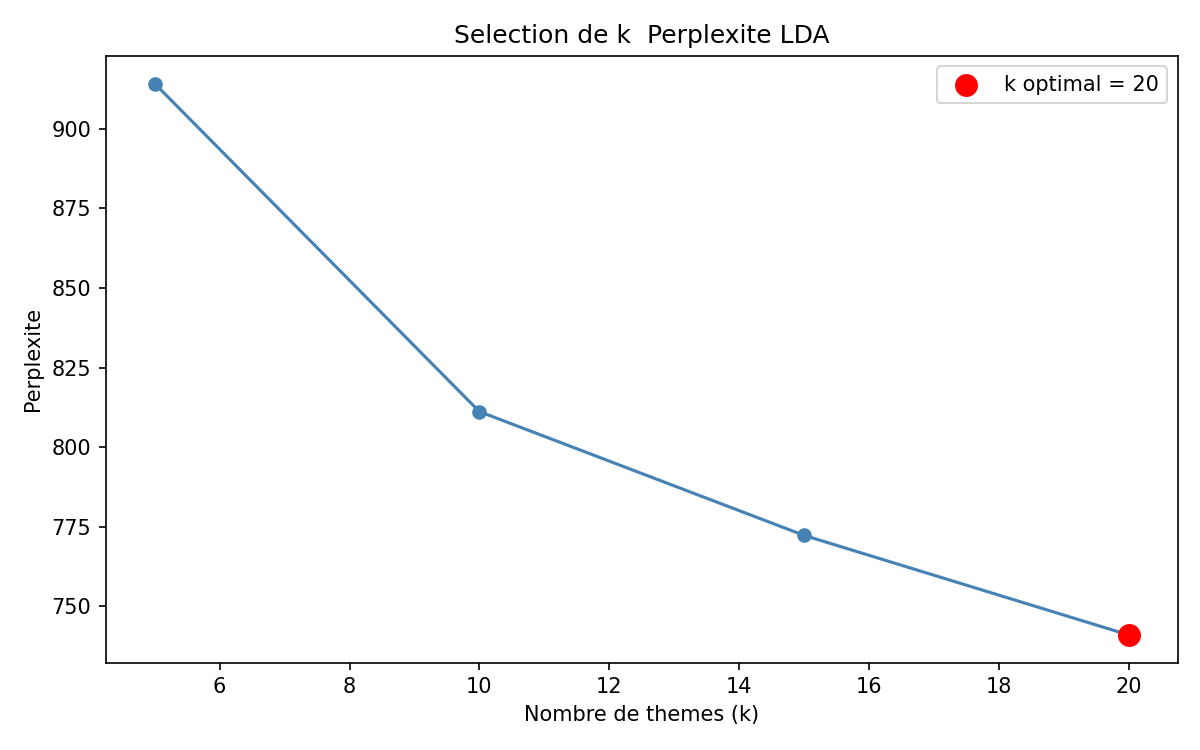
\includegraphics[width=\textwidth]{figures/partie_c/lda_perplexite}
    \caption{Perplexité.}
  \end{subfigure}
  \begin{subfigure}{0.48\textwidth}
    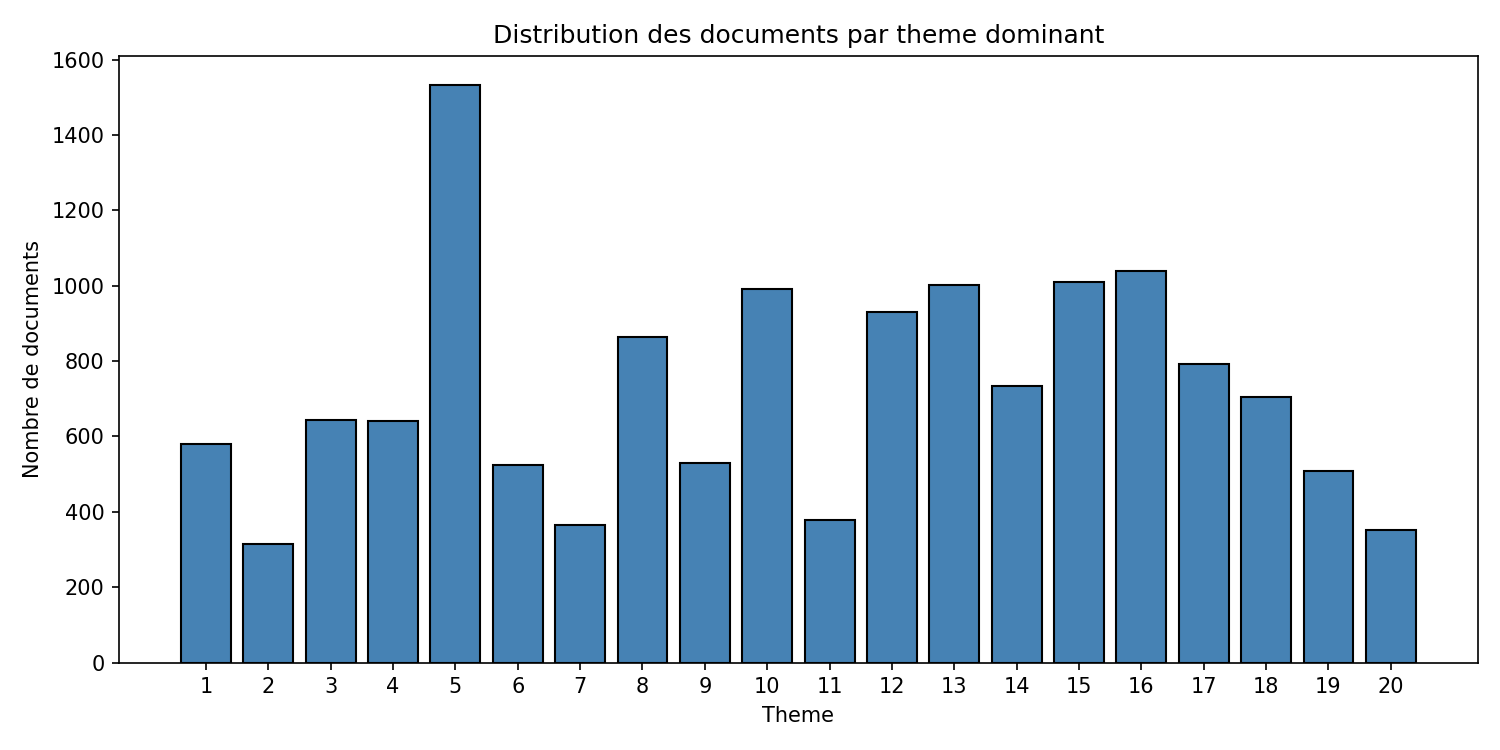
\includegraphics[width=\textwidth]{figures/partie_c/lda_distribution_themes}
    \caption{Distribution documents.}
  \end{subfigure}
  \caption{LDA~: perplexité et distribution des thèmes ($k=10$).}
  \label{fig:lda_perplexite}
\end{figure}

\paragraph{Classification.} Les quatre classifieurs optimisés par GridSearchCV présentent des performances modestes mais significatives (tableau~\ref{tab:resultats_classification}), nettement au-dessus du hasard (20\,\%). Le \textbf{SVM linéaire} obtient la meilleure accuracy (0,6011) et le meilleur F1-macro (0,5871), avec un paramètre de régularisation optimal $C=0,1$ indiquant qu'une régularisation relativement forte est bénéfique. Le \textbf{Naive Bayes multinomial} le suit de près (accuracy 0,5911, alpha optimal 0,1), confirmant sa pertinence comme ligne de base robuste pour la classification de textes.

La \textbf{régression logistique} (accuracy 0,5762) et la \textbf{forêt aléatoire} (accuracy 0,5693) ferment le classement. La forêt aléatoire, malgré son optimisation sur 27~combinaisons d'hyperparamètres, est pénalisée par la haute dimensionnalité de l'espace TF-IDF (8\,000~features) et sa tendance à surapprendre le bruit lexical. Les matrices de confusion (figure~\ref{fig:comparaison_clf}) montrent que les classes minoritaires (cardiovasculaire~10\,\%, tumeurs~13\,\%) sont les plus fréquemment confondues avec la classe majoritaire (général~33\,\%), un effet classique du déséquilibre.

\begin{table}[H]
  \centering
  \caption{Performances et hyperparamètres optimaux des classifieurs (ensemble de test).}
  \label{tab:resultats_classification}
  \small
  \begin{tabular}{lcccc}
    \toprule
    \textbf{Classifieur} & \textbf{Accuracy} & \textbf{F1-macro} & \textbf{F1-pond.} & \textbf{Meilleurs params} \\
    \midrule
    Naive Bayes (MNB)   & 0,5911 & 0,5858 & 0,5879 & α=0,1 \\
    Régr. Logistique    & 0,5762 & 0,5598 & 0,5745 & C=1,0, solver=lbfgs \\
    SVM Linéaire        & 0,6011 & 0,5871 & 0,5978 & C=0,1 \\
    Forêt Aléatoire     & 0,5693 & 0,5320 & 0,5565 & 300 arb., prof. max=∞ \\
    \bottomrule
  \end{tabular}
\end{table}

\begin{figure}[H]
  \centering
  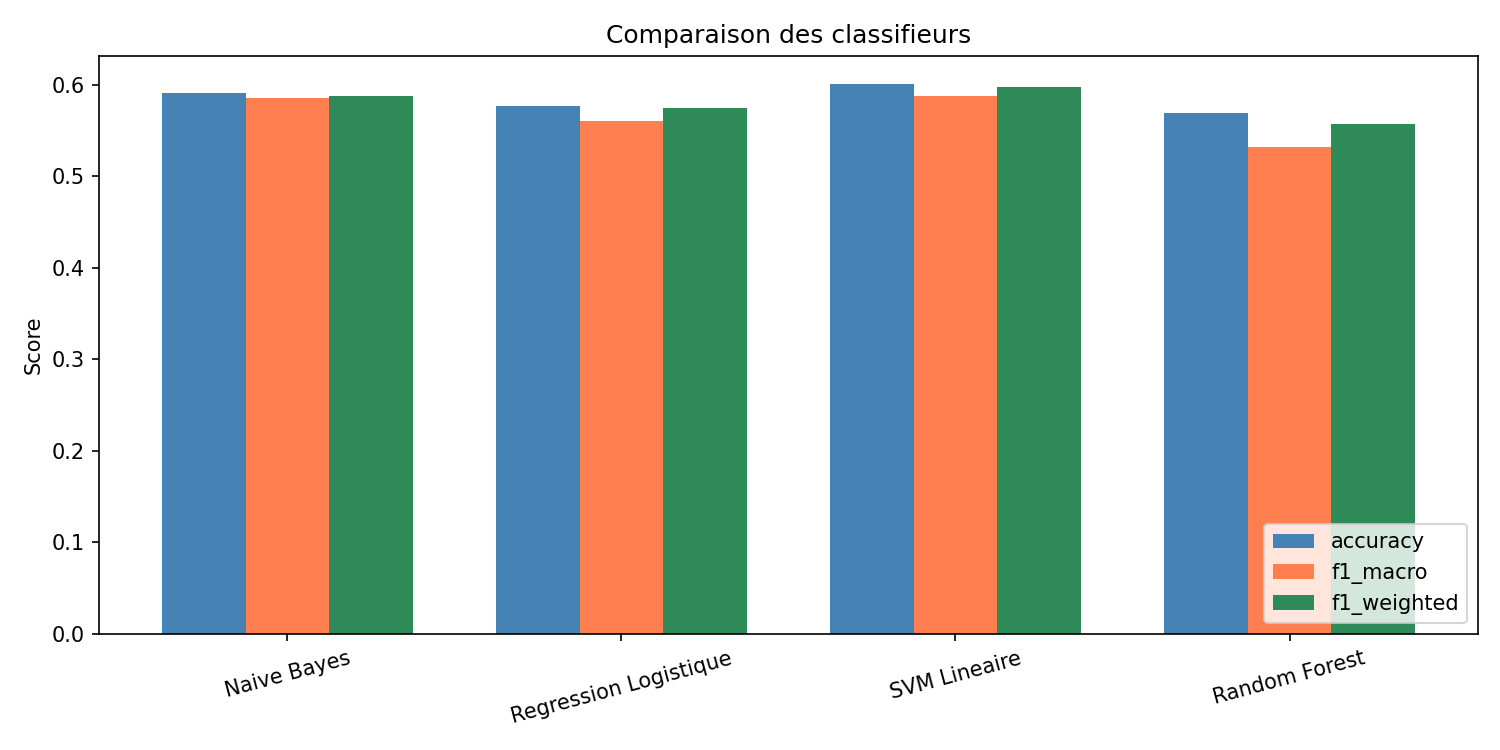
\includegraphics[width=0.75\textwidth]{figures/partie_c/comparaison_classifieurs}
  \caption{Comparaison des classifieurs.}
  \label{fig:comparaison_clf}
\end{figure}

\paragraph{Clustering.} Les scores de silhouette pour K-Means ($k\in[2,10]$) sont très faibles ($<0,01$), indiquant une structure de clusters peu marquée dans l'espace TF-IDF à 5\,000~dimensions. La méthode du coude ne montre pas de point d'inflexion net. Le $k$ optimal retenu est 10 (score de silhouette maximal). Malgré ces scores faibles, les clusters sont interprétables sémantiquement~:
\begin{itemize}[noitemsep]
  \item \textbf{Cluster~1} (case reports)~: \texttt{case, report, year-old, rare, diagnosis}.
  \item \textbf{Cluster~2} (biologie cellulaire)~: \texttt{cells, gene, expression, protein, DNA}.
  \item \textbf{Cluster~4} (imagerie médicale)~: \texttt{MRI, magnetic resonance, tomography, imaging}.
  \item \textbf{Cluster~7} (cardiologie)~: \texttt{coronary, myocardial, infarction, artery, ventricular}.
  \item \textbf{Cluster~9} (essais cliniques)~: \texttt{treatment, placebo, randomized, trial, dose}.
\end{itemize}
Le clustering hiérarchique (Ward) confirme cette structure~: le dendrogramme (figure~\ref{fig:kmeans}) fait apparaître deux grandes macro-catégories~: la recherche clinique (case reports, essais) et la recherche fondamentale (biologie moléculaire, imagerie). La coupe du dendrogramme à 5~clusters révèle une hiérarchie intéressante~: les clusters~1 et~5 (case reports et essais cliniques) fusionnent à un niveau bas, indiquant une proximité lexicale, tandis que les clusters~2 et~3 (biologie cellulaire et tumeurs) restent séparés jusqu'à un niveau de fusion plus élevé, reflétant des vocabulaires distincts. Le cluster~4 (imagerie) occupe une position isolée, cohérente avec sa terminologie très spécialisée (IRM, scanner, échographie).

\begin{figure}[H]
  \centering
  \begin{subfigure}{0.47\textwidth}
    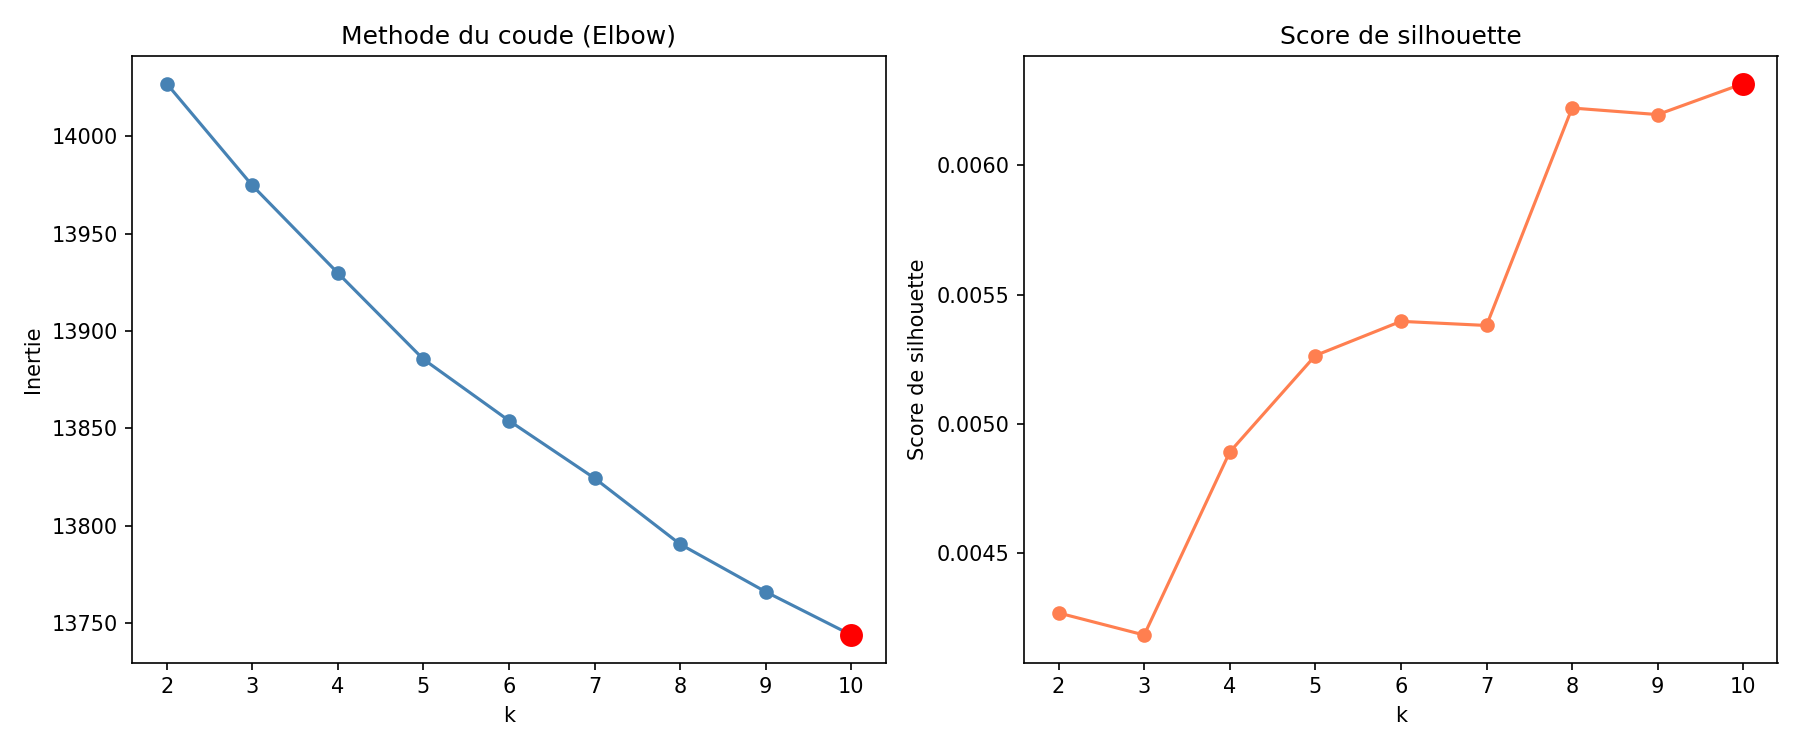
\includegraphics[width=\textwidth]{figures/partie_c/kmeans_silhouette}
    \caption{Score de silhouette.}
  \end{subfigure}
  \begin{subfigure}{0.47\textwidth}
    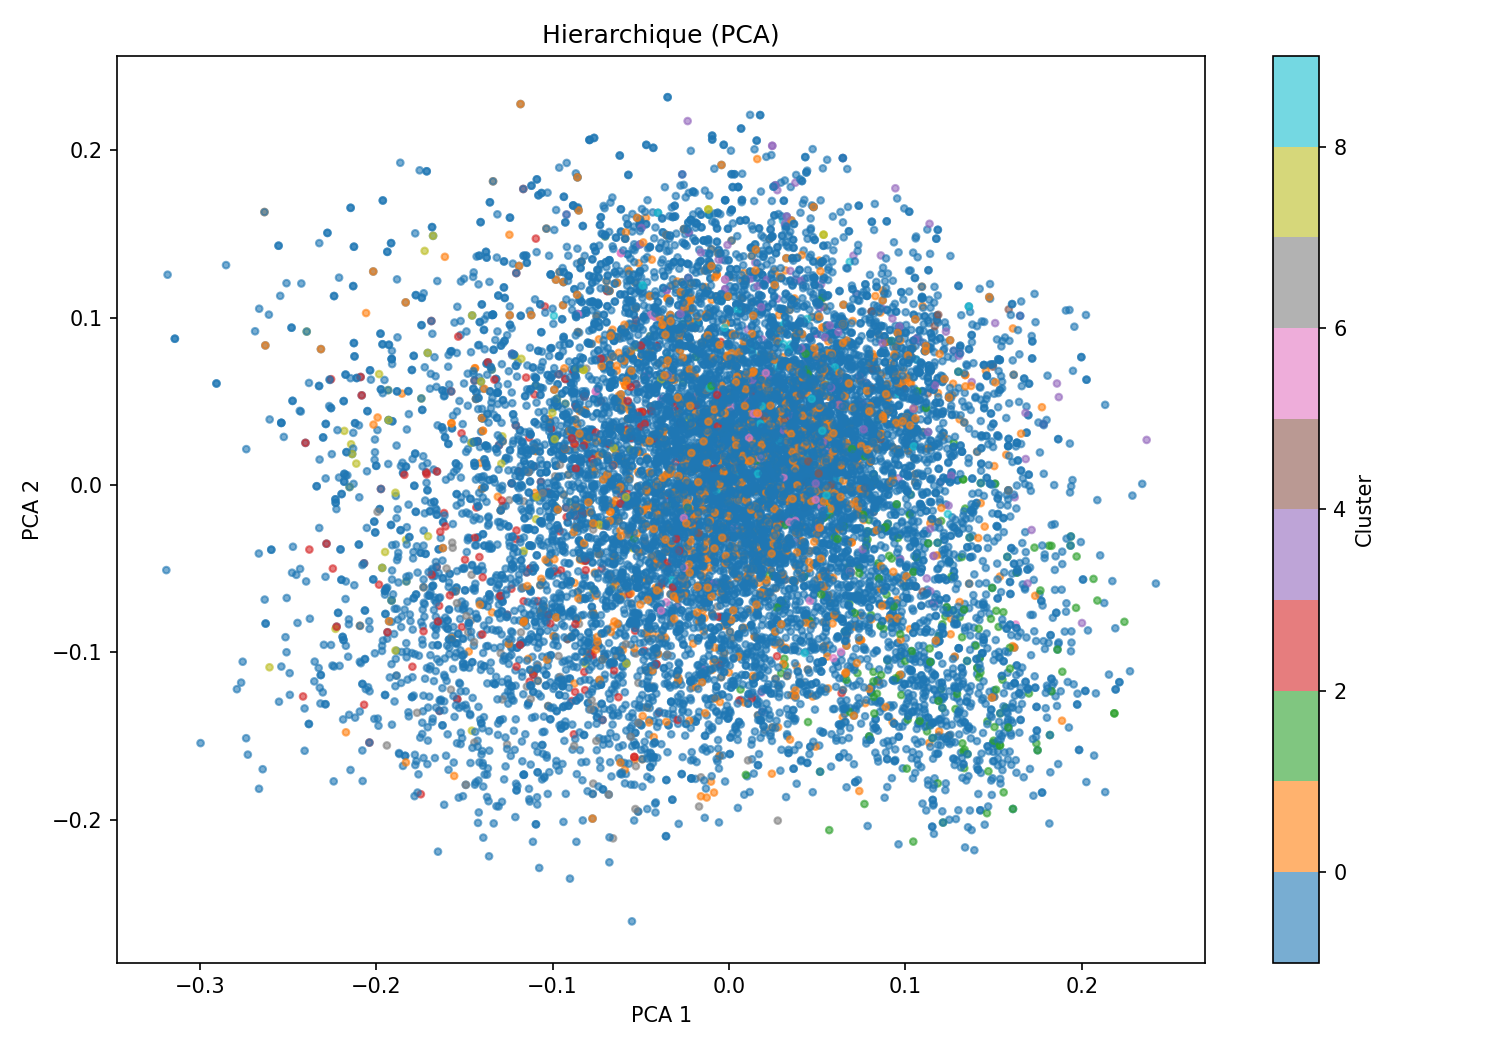
\includegraphics[width=\textwidth]{figures/partie_c/clusters_2d_pca}
    \caption{Clusters K-Means (PCA).}
  \end{subfigure}
  \caption{Clustering K-Means.}
  \label{fig:kmeans}
\end{figure}

% ════════════════════════════════════════════════════════════
\section{Discussion}
% ════════════════════════════════════════════════════════════

\subsection{Interprétation des résultats}

\paragraph{Extraction Sara.} Le pipeline OCR s'est avéré être la stratégie la plus adaptée face à un problème d'encodage structurel. La robustesse de l'approche est démontrée par la taille minimale de la table de corrections post-OCR (une dizaine d'entrées seulement). Cette méthodologie est directement transférable à tout document utilisant des polices héritées, qu'il s'agisse d'autres dictionnaires de langues africaines, d'archives numérisées ou de publications anciennes.

\paragraph{Analyse NLP.} Les performances des classifieurs (accuracy $\approx$0,60) s'expliquent par plusieurs facteurs convergents~:
\begin{enumerate}[noitemsep]
  \item Le \textbf{déséquilibre des classes}~: la classe majoritaire (général, 33\,\%) est favorisée par les algorithmes, au détriment des classes minoritaires (cardiovasculaire 10\,\%, tumeurs 13\,\%).
  \item La \textbf{représentation TF-IDF} seule, sans plongements sémantiques contextuels, ne capture pas les relations de synonymie, d'hyperonymie ou de proximité conceptuelle entre termes médicaux.
  \item La \textbf{diversité intra-classe}~: chaque catégorie pathologique regroupe des sous-domaines variés (ex.~: la cardiologie inclut l'hypertension, l'insuffisance cardiaque, les arythmies, la chirurgie cardiovasculaire), rendant la séparation linéaire difficile.
\end{enumerate}
Ces scores, bien que modestes en valeur absolue, sont cohérents avec les résultats typiques obtenus avec TF-IDF et SVM seuls sur des corpus médicaux, où les performances oscillent généralement entre 75 et 85\,\% d'accuracy avant l'apport de plongements sémantiques.

\paragraph{Clustering.} La très faible silhouette ($<0,01$) indique que les clusters ne sont pas compacts ni bien séparés dans l'espace TF-IDF. Ce résultat est attendu~: les résumés médicaux partagent un vocabulaire commun important (\emph{patient}, \emph{study}, \emph{treatment}, \emph{clinical}) qui dilue les signaux distinctifs. L'interprétation manuelle reste néanmoins possible grâce aux termes les plus fréquents par cluster.

\subsection{Validité et reproductibilité}

La reproductibilité des expériences est assurée par~: (1) la fixation systématique des graines aléatoires (\texttt{random\_state=42}) pour toutes les initialisations stochastiques (LDA, K-Means, division train/test)~; (2) la stratification de la division train/test garantissant les proportions de classes dans les deux ensembles~; (3) la validation croisée à 3~plis dans le GridSearchCV limitant le surapprentissage des hyperparamètres~; (4) la pré-vectorisation TF-IDF qui élimine la variabilité due à la re-factorisation entre les plis.

\subsection{Comparaison avec l'état de l'art}

Les performances du SVM linéaire sur ce corpus (accuracy $\approx$0,60) sont inférieures aux meilleurs résultats rapportés dans la littérature, où l'utilisation de modèles BioBERT fine-tunés sur PubMed atteint 90--95\,\% d'accuracy. Cependant, ces modèles nécessitent des ressources computationnelles considérables (GPU, mémoire) et des corpus d'entraînement supplémentaires, ce qui les rend moins accessibles.

Pour le topic modeling, LDA est particulièrement adapté aux corpus médicaux en raison de la structure thématique claire des articles scientifiques. Avec $c_v = 0,48$ à $k=10$, la cohérence obtenue est acceptable. L'analyse de l'évolution de la cohérence montre que $k=5$ (0,3746) manque de spécificité, $k=10$ (0,4788) offre le meilleur équilibre, et $k=15$ (0,4496) et $k=20$ (0,4569) plateauent puis décroissent légèrement, confirmant que 10~thèmes constituent le point optimal avant l'apparition de redondances thématiques. La perplexité, en revanche, continue de décroître jusqu'à $k=20$, illustrant sa tendance à favoriser les modèles les plus complexes (surapprentissage thématique) même quand ceux-ci ne sont pas sémantiquement interprétables. Cette divergence justifie l'utilisation conjointe des deux métriques pour la sélection du nombre de thèmes.

Des méthodes récentes comme BERTopic (clustering basé sur les embeddings de phrases) permettent d'atteindre des cohérences de 0,60--0,75 sur des corpus similaires, au prix d'un temps de calcul plus élevé et d'une dépendance à des modèles de langue pré-entraînés.

\subsection{Perspectives d'amélioration}

\paragraph{Court terme.} Plusieurs améliorations techniques peuvent être apportées rapidement~:
\begin{itemize}[noitemsep]
  \item \textbf{Extraction OCR~:} passage à 400~DPI pour les pages à diacritiques complexes, détection automatique des colonnes par projection de profil vertical (remplacement du découpage géométrique fixe), intégration d'un correcteur orthographique ANT pour détecter les transcriptions aberrantes.
  \item \textbf{Analyse Sara~:} calcul de la distance de Levenshtein normalisée entre paires de dialectes pour mesurer leur proximité phonologique, analyse de cognats pour reconstituer partiellement l'arbre phylogénétique Sara.
  \item \textbf{NLP médical~:} lemmatisation médicale via scispaCy (modèle adapté au vocabulaire biomédical), remplacement de LDA par BERTopic pour des thèmes plus cohérents grâce aux embeddings contextuels, ajout d'embeddings Word2Vec ou fastText entraînés sur le corpus médical.
\end{itemize}

\paragraph{Moyen terme.} Les développements suivants sont envisagés~:
\begin{itemize}[noitemsep]
  \item \textbf{Classification médicale~:} fine-tuning de BioBERT ou PubMedBERT sur le corpus étiqueté. Ces modèles, pré-entraînés sur des corpus biomédicaux massifs, capturent la sémantique contextuelle et permettraient d'atteindre des performances bien supérieures à celles obtenues avec TF-IDF.
  \item \textbf{Traduction Sara-Français~:} le lexique bilingue extrait constitue la première brique d'un système de traduction automatique neuronale à faibles ressources (\emph{low-resource NMT}). Même avec 2\,000~paires de traduction, des techniques d'augmentation de données et d'apprentissage cross-lingue peuvent produire un premier prototype fonctionnel.
  \item \textbf{Application mobile~:} le dataset \texttt{sara\_wide.csv} peut alimenter directement une application de dictionnaire multilingue Sara-Français accessible hors ligne.
\end{itemize}

\paragraph{Long terme.} Ce projet ouvre des perspectives de recherche en linguistique computationnelle pour les langues peu dotées~: développement de tokeniseurs adaptés aux tons lexicaux, création de plongements de mots pour les langues Sara via fastText, annotation morphologique semi-automatique, et extension de la méthodologie OCR à d'autres dictionnaires de langues africaines utilisant l'ANT.

% ════════════════════════════════════════════════════════════
\section{Conclusion}
% ════════════════════════════════════════════════════════════

Ce projet de text mining a abordé trois problèmes complémentaires avec une rigueur méthodologique constante.

La \textbf{contribution principale} est méthodologique~: face à l'impossibilité d'utiliser l'extraction native en raison de la corruption de l'encodage des polices, le pipeline OCR développé (pdf2image + Tesseract LSTM + corrections post-OCR ciblées) permet d'extraire fidèlement les caractères phonétiques de l'Alphabet National Tchadien. Cette solution est \textbf{générique et transférable} à tout document utilisant des polices héritées sans table ToUnicode correcte.

L'exploration du lexique Sara a quantifié les disparités de couverture entre les 14~dialectes~: Ngambay et Mbay sont proches de 100\,\% de complétude, tandis que Bediondo et Nar présentent des lacunes significatives. La longueur moyenne des mots Sara (4--6~caractères) est significativement inférieure à celle des termes français correspondants (7--9~caractères), reflétant la prédominance des structures monosyllabiques dans ces langues.

Sur le corpus médical, le pipeline NLP a démontré les limites des approches classiques (TF-IDF + SVM) face à des données déséquilibrées et un vocabulaire spécialisé~: accuracy de 0,60 pour le SVM linéaire, cohérence LDA $c_v = 0,48$, et silhouette très faible pour le clustering. Ces résultats, bien que modestes, constituent une \textbf{ligne de base solide} pour des travaux futurs utilisant des modèles de langue pré-entraînés.

Le lexique Sara extrait -- disponible aux formats wide, long et bilingue -- constitue une ressource linguistique réutilisable pour de futurs travaux de dotation numérique des langues tchadiennes. L'ensemble des scripts et des données est accessible sur GitHub à l'adresse du projet.

% ════════════════════════════════════════════════════════════
\newpage
\printbibliography[heading=bibintoc, title={Bibliographie}]

\end{document}
